\documentclass[dvipsnames]{standalone}
\usepackage{tikz}

\usetikzlibrary{positioning, arrows, arrows.meta}
\usetikzlibrary{shapes,arrows,chains}


\colorlet{G1}{SkyBlue!50}
\colorlet{G2}{LimeGreen!50}
\colorlet{G3}{RedOrange!60}

\begin{document}

    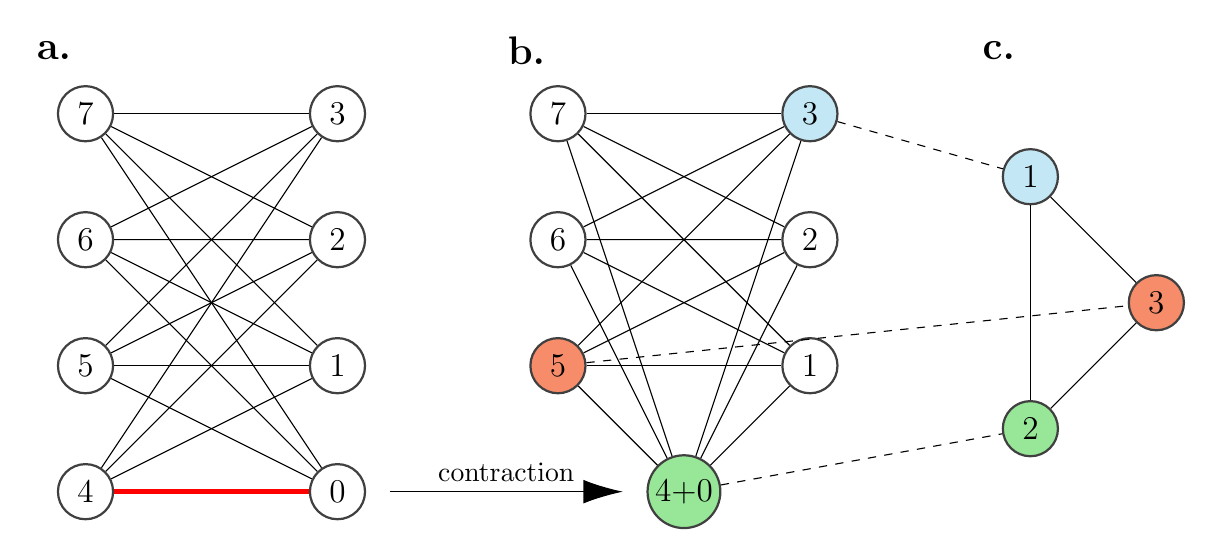
\begin{tikzpicture}[
        scale=0.4,
        coupler/.style={draw},
        qubit/.style={circle, thick, font={\large}, fill=White,draw=darkgray,minimum size=7mm, inner sep=0.5mm},
        hidden/.style={opacity=0.0},
        internal/.style={color=black, thin},    
        highlight/.style={color=red, ultra thick},
        assignment/.style={dashed}
    ]
    \node at (-1, 14) {\Large \textbf{a.}};
    \node[qubit, hidden] (0) at (8.0, 0.0) { 0 };
    \node[qubit, hidden] (4) at (0.0, 0.0) { 4 };
    \node[qubit, hidden] (5) at (0.0, 4.0) { 5 };
    \node[qubit, hidden] (6) at (0.0, 8.0) { 6 };
    \node[qubit, hidden] (7) at (0.0, 12.000000000000002) { 7 };
    \node[qubit, hidden] (1) at (8.0, 4.0) { 1 };
    \node[qubit, hidden] (2) at (8.0, 8.0) { 2 };
    \node[qubit, hidden] (3) at (8.0, 12.000000000000002) { 3 };
    \path[coupler, highlight] (0) edge (4);
    \path[coupler, internal] (0) edge (5);
    \path[coupler, internal] (0) edge (6);
    \path[coupler, internal] (0) edge (7);
    \path[coupler, internal] (4) edge (1);
    \path[coupler, internal] (4) edge (2);
    \path[coupler, internal] (4) edge (3);
    \path[coupler, internal] (5) edge (1);
    \path[coupler, internal] (5) edge (2);
    \path[coupler, internal] (5) edge (3);
    \path[coupler, internal] (6) edge (1);
    \path[coupler, internal] (6) edge (2);
    \path[coupler, internal] (6) edge (3);
    \path[coupler, internal] (7) edge (1);
    \path[coupler, internal] (7) edge (2);
    \path[coupler, internal] (7) edge (3);

    \node[qubit] (0-front) at (8.0, 0.0) { 0 };
    \node[qubit] (4-front) at (0.0, 0.0) { 4 };
    \node[qubit] (5-front) at (0.0, 4.0) { 5 };
    \node[qubit] (6-front) at (0.0, 8.0) { 6 };
    \node[qubit] (7-front) at (0.0, 12.000000000000002) { 7 };
    \node[qubit] (1-front) at (8.0, 4.0) { 1 };
    \node[qubit] (2-front) at (8.0, 8.0) { 2 };
    \node[qubit] (3-front) at (8.0, 12.000000000000002) { 3 };

    \begin{scope}[xshift=15cm][name prefix=contracted]    
    \node at (-1, 14) {\Large \textbf{b.}};
    \node[qubit, hidden] (40) at (4.0, 0.0) { 4 };
    \node[qubit, hidden] (5) at (0.0, 4.0) { 5 };
    \node[qubit, hidden] (6) at (0.0, 8.0) { 6 };
    \node[qubit, hidden] (7) at (0.0, 12.000000000000002) { 7 };
    \node[qubit, hidden] (1) at (8.0, 4.0) { 1 };
    \node[qubit, hidden] (2) at (8.0, 8.0) { 2 };
    \node[qubit, hidden] (3) at (8.0, 12.000000000000002) { 3 };    
    \path[coupler, internal] (40) edge (5);
    \path[coupler, internal] (40) edge (6);
    \path[coupler, internal] (40) edge (7);
    \path[coupler, internal] (40) edge (1);
    \path[coupler, internal] (40) edge (2);
    \path[coupler, internal] (40) edge (3);
    \path[coupler, internal] (5) edge (1);
    \path[coupler, internal] (5) edge (2);
    \path[coupler, internal] (5) edge (3);
    \path[coupler, internal] (6) edge (1);
    \path[coupler, internal] (6) edge (2);
    \path[coupler, internal] (6) edge (3);
    \path[coupler, internal] (7) edge (1);
    \path[coupler, internal] (7) edge (2);
    \path[coupler, internal] (7) edge (3);
    %\node[qubit] (0-front) at (8.0, 0.0) { 0 };
    \node[qubit, fill=G2] (40-front) at (4.0, 0.0) { 4+0 };
    \node[qubit, fill=G3] (5-front) at (0.0, 4.0) { 5 };
    \node[qubit] (6-front) at (0.0, 8.0) { 6 };
    \node[qubit] (7-front) at (0.0, 12.000000000000002) { 7 };
    \node[qubit] (1-front) at (8.0, 4.0) { 1 };
    \node[qubit] (2-front) at (8.0, 8.0) { 2 };
    \node[qubit, fill=G1] (3-front) at (8.0, 12.000000000000002) { 3 };
    \end{scope}
    
    \begin{scope}[xshift=30cm]
    \node at (-1, 14) {\Large \textbf{c.}};
    \node[qubit, fill=G1] (G1) at (0, 10) { 1 };
    \node[qubit, fill=G2] (G2) at (0, 2) { 2 };
    \node[qubit, fill=G3] (G3) at (4, 6) { 3 };

    \path (G1) edge (G2);
    \path (G2) edge (G3);
    \path (G3) edge (G1);
    \end{scope}

    \path[assignment] (40-front) edge (G2);
    \path[assignment] (5) edge (G3);
    \path[assignment] (3) edge (G1);

    \path[-{Latex[length=5mm,width=3mm]}, shorten <= 0.3cm, shorten >= 0.3cm] 
    (0) edge node[midway, above]  {contraction} (40-front);
    \end{tikzpicture}

\end{document}